%%%%%%%%%%%%%%%%%%%%%%%%%%%%%%%%%%%%%%%%%%%%%%%%%%%%%%%%%%%%%%%%%%
%%  ~ Trabajo de Fin de Grado - Universidad de Vigo (ESEI) ~    %%
%% Autor: Diego Enrique Fontán Lorenzo                          %%
%% Tutor: Miguel Ramón Díaz-Cacho Medina                        %%
%% Convocatoria: Julio 2020/21                                  %%
%% Título: Framework de automatización de auditorías Red Team   %%
%%%%%%%%%%%%%%%%%%%%%%%%%%%%%%%%%%%%%%%%%%%%%%%%%%%%%%%%%%%%%%%%%%

%%%%%%%%%%%%%%%%%%%%%%%%%%%%%
%% User guide
%%%%%%%%%%%%%%%%%%%%%%%%%%%%%

\chapter{Manual de usuario} \label{anx:manual}

En este anexo se describen los aspectos básicos de la aplicación, como la estructura de los directorios, la guía de instalación, la creación de \textit{ingredientes} y el uso básico de la misma.\sn

El código de la aplicación está disponible \textit{online} en la siguiente dirección web:\sn

\hfil\url{https://github.com/cosasdepuma/Masterchef}\hfil\n

\section{Estructura de los directorios} \label{sec:folderstructure}

Los archivos y directorios más relevantes del proyecto se encuentran estructurados siguiendo el esquema mostrado a continuación.\sn

\subsection{Directorio raíz} \label{sub:rootdir}

El \textbf{directorio raíz} cuenta con tres carpetas:\sn

\textbf{.github/}: Archivos pertenecientes a la documentación de \textit{GitHub}.

\textbf{backend/}: Código fuente del servidor.

\textbf{frontend/}: Código fuente de la interfaz.\sn

También cuenta con los siguientes ficheros:\sn

\textbf{.gitignore}: Archivos ignorados por \textit{GitHub}.

\textbf{.dockerignore}: Archivos ignorados por \textit{Docker}.

\textbf{Makefile}: Parámetros de auto-compilación.

\textbf{Dockerfile}: Archivo para compilar y desplegar la aplicación usando contenedores.

\textbf{docker-compose.yml}: Fichero para orquestar contenedores.

\textbf{version}: Versión actual del programa.

\textbf{swagger.yml}: Documentación de la \textit{API}.

\textbf{README.md}: Documentación del repositorio.

\textbf{LICENSE}: Licencia del repositorio.\sn

\subsection{Directorio \textit{frontend}} \label{sub:frontenddir}.

La carpeta \textit{frontend} cuenta con los siguientes archivos:\sn

\textbf{.browserslistrc}: Navegadores soportados por la interfaz.

\textbf{babel.config.js}: Archivo de configuración de \textit{Babel}.

\textbf{compile.js}: \textit{Script} para añadir el \textit{frontend} en ficheros \textit{.go}.

\textbf{package.json}: Archivo de configuración del \textit{frontend}.

\textbf{patches.js}: \textit{Script} para corregir errores en las dependencias.

\textbf{vue.config.js}: Archivo de configuración de \textit{Vue}.

\textbf{yarn.lock}: Versiones e integridad de las dependencias de desarrollo.\sn

Respecto a las carpetas, existen dos dentro del directorio \textit{frontend}: \textbf{public/} (con los archivos estáticos, como la plantilla \textit{HTML}) y \textbf{src/}, con el código fuente relativo al núcleo de la interfaz. Esta última está estructurada de la siguiente manera:\sn

\textbf{App.vue}: Vista principal de la aplicación.

\textbf{main.js}: Entrada de la aplicación, encargada de montar la vista.

\textbf{assets/}: Archivos auxiliares. Contiene las especificaciones de los nodos.

\textbf{components/}: Componentes visuales de la interfaz.

\textbf{ingredients/}: Archivos relativos a la interpretación de los nodos.

\textbf{scripts/}: Otros ficheros de \textit{Javascript}. Contiene la lógica del \textbf{editor/}, formado a su vez por \textbf{plugins/} y \textbf{components/} (tipos de controles). También provee de funciones auxiliares (\textbf{helpers/}), iconos (\textbf{icons/}) y validaciones (\textbf{validator/}).

\subsection{Directorio \textit{backend}} \label{sub:backenddir}.

La carpeta \textit{backend} contiene los siguientes directorios y archivos:\sn

\textbf{go.mod}: Dependencias de desarrollo.

\textbf{go.sum}: Versiones e integridad de las dependencias de desarrollo.

\textbf{main.go}: Punto de entrada de la aplicación si se ejecuta mediante un binario.

\textbf{cmd/}: Punto de entrada de la aplicación si se instala con \textit{go get}.

\textbf{public/}: Archivo auto-generados por el \textit{frontend}.

\textbf{app/}: Código fuente relativo al núcleo del servidor.\sn

La carpeta \textbf{app/} está estructurada de la siguiente forma:\sn

\textbf{config/}: Parámetros de configuración por defecto y variables de entorno.

\textbf{helpers/}: Funciones auxiliares.

\textbf{providers/}: Código para la obtención de información mediante fuentes abiertas.

\textbf{server/}: Archivos relativos al servidor \textit{HTTP}.\sn

La carpeta \textbf{server/} consta, a su vez, de los archivos \textbf{server.go} (servicio \textit{HTTP}) y \textbf{router.go} (enrutador). También cuenta con los directorios \textbf{client/} (cliente \textit{HTTP}), \textbf{middlewares/} (funciones auxiliares del enrutador) y \textbf{routes/} (rutas de la \textit{API}).\n

\section{Compilación} \label{sec:compilation}

En entornos \textit{*nix}, la compilación se puede llevar a cabo por medio del comando \textbf{make}, gracias a las reglas descritas en el archivo \textit{Makefile}.\sn

Por el contrario, si se desea realizar una compilación manual o no se dispone de las herramientas necesarias para ejecutarla de manera automatizada, se puede realizar el siguiente procedimiento:\sn

\begin{quote}
----- Interfaz

yarn --cwd frontend/ install

yarn --cwd frontend/ run compile

----- Servidor

cd backend/

go build main.go

----- Opcional

upx -o masterchef main\n
\end{quote}

\section{Instalación} \label{sec:installation}

La aplicación está disponible de modo portable. Se puede descargar directamente desde el apartado \textit{Releases} del repositorio \textit{online}. Su tamaño aproximado es de 1,9M para la versión 0.1.0.\sn

Si se desea instalar, es posible realizarlo mediante el comando\footnote{Es necesario tener \textit{Golang 1.16} instalado en el sistema}:\sn

\hfil go get -u github.com/cosasdepuma/Masterchef \hfil\n

\section{Requisitos mínimos} \label{sec:minimumrequirements}

La aplicación no cuenta con requisitos mínimos. Es posible compilarla para cualquier sistema operativo y arquitectura. Tampoco depende de ficheros o programas de terceros.\sn

En el caso de ejecutar tareas de recopilación de información o que tengan como objetivo un activo externo, puede ser necesaria una conexión a Internet.\sn

\textbf{Nota}: Actualmente el editor de nodos no funciona correctamente en dispositivos móviles o \textit{tablets}.\n

\section{Uso de la aplicación} \label{sec:usage}

A continuación, se detalla el uso de la aplicación. Se divide en tres partes: ejecución, llamadas a la \textit{API} y creación de nuevos nodos.\n

\subsection{Ejecución} \label{sub:execution}

Para iniciar el servidor, solamente basta con lanzar el programa \fig{execdefault}. Si se ejecuta desde una terminal, se pueden configurar los parámetros mediante las variables de entorno \textbf{MC\_ADDR} y \textbf{MC\_THREADS} \fig{execenv}:\sn

\begin{figure}[H]
     \centering
     \begin{subfigure}[b]{0.3\textwidth}
         \centering
         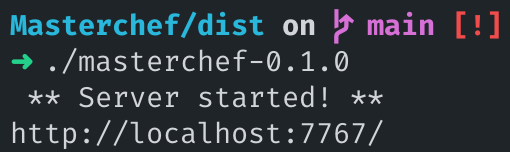
\includegraphics[width=\textwidth]{img/tables/38_Running.png}
         \caption{Ejecución estándar.}
         \label{fig:execdefault}
     \end{subfigure}
     \begin{subfigure}[b]{0.6\textwidth}
         \centering
         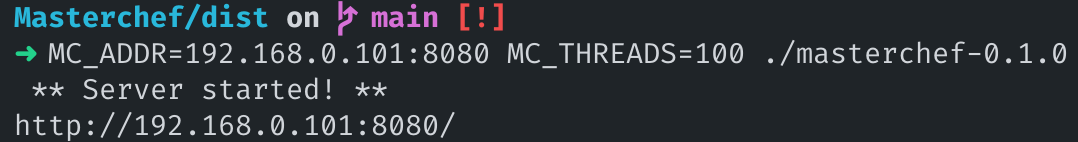
\includegraphics[width=\textwidth]{img/tables/39_Running-Env.png}
         \caption{Ejecución personalizada.}
         \label{fig:execenv}
     \end{subfigure}
    \caption{Ejecución de la aplicación.}
    \label{fig:exec}
\end{figure}

También es posible levantar el servicio usando \textit{Docker} gracias al archivo \textit{Dockerfile}.\sn

Una vez ejecutado, será necesario acceder a la dirección definida con el fin de visualizar la interfaz gráfica \fig{justtheinterface}. La \textit{URL} por defecto es \url{http://127.0.0.1:7767/}.\sn

\begin{figure}[H]
    \centering
    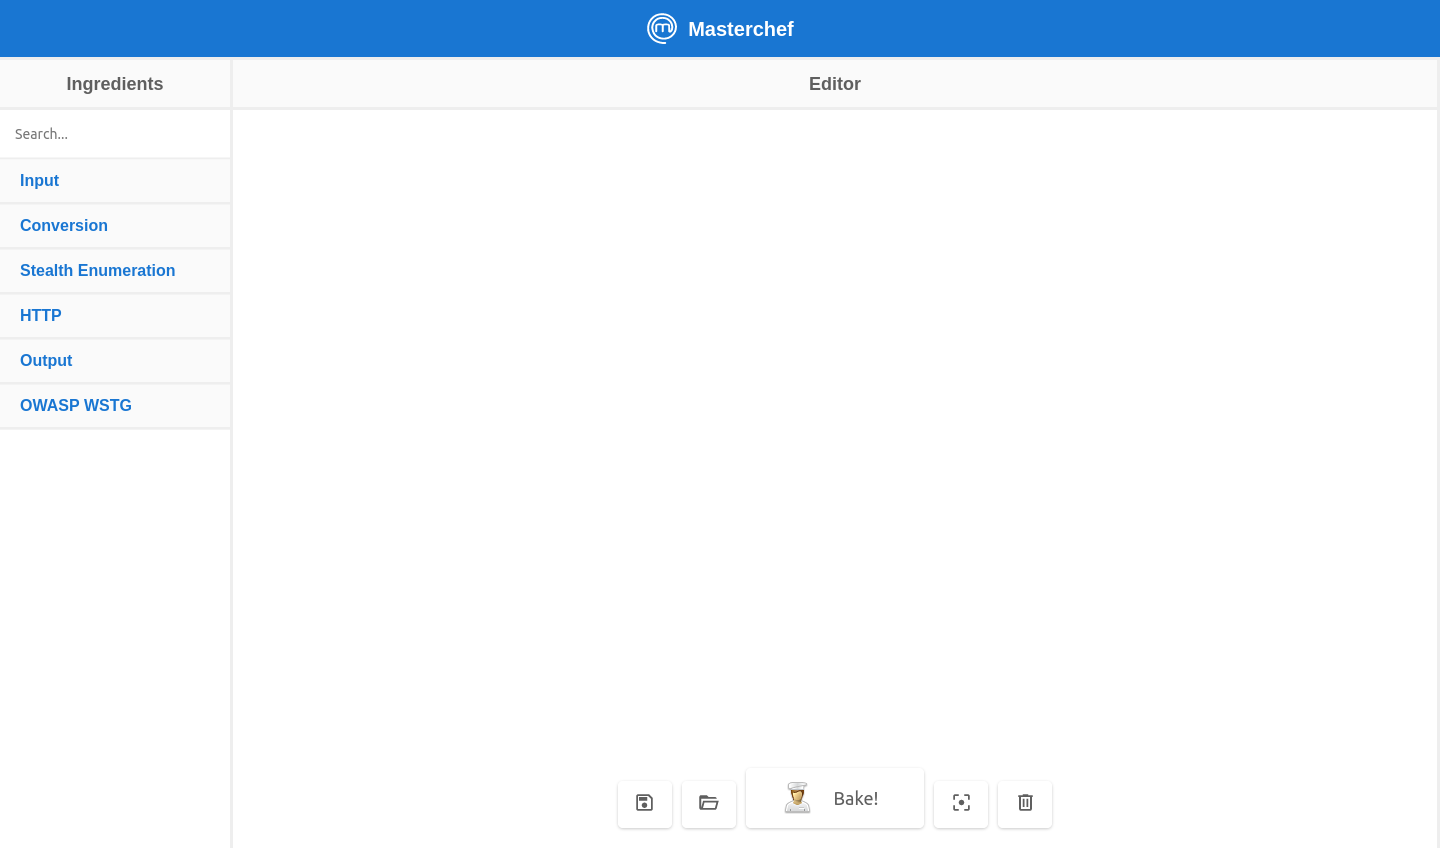
\includegraphics[width=15cm]{img/tables/40_Interface.png}
    \caption{Interfaz de la aplicación.}
    \label{fig:justtheinterface}
\end{figure}

El panel lateral izquierdo cuenta con los nodos disponibles (denominados \textit{ingredientes}). Están agrupados por categorías. Se puede desplegar u ocultar una categoría pulsando sobre ella. También contiene un buscador que permite filtrar los nodos por palabras clave. Es posible obtener la descripción de un ingrediente depositando el cursor encima del mismo \fig{ingrdesc}.\sn

\begin{figure}[H]
    \centering
    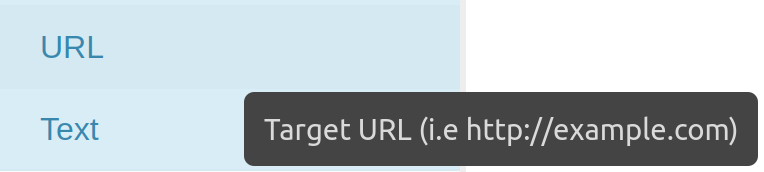
\includegraphics[width=10cm]{img/tables/41_Ingredient-Tooltip.png}
    \caption{Descripción del ingrediente.}
    \label{fig:ingrdesc}
\end{figure}

Los ingredientes pueden ser añadidos al editor arrastrándolos sobre él. Éstos constan de tres partes fundamentales \fig{ingredientskeleton}: los datos de entrada (a la izquierda), los datos de salida (a la derecha) y los controles (en el centro). Cada dato lleva asociado un tipo específico que limita su conexión con otros nodos. Para comprobar el tipo de conexión, basta con mantener el cursor encima del conector.\sn

\begin{figure}[H]
    \centering
    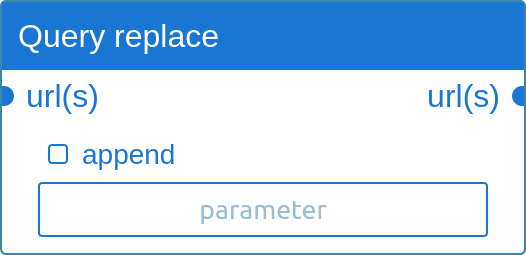
\includegraphics[width=8cm]{img/tables/42_Ingredient.png}
    \caption{Estructura de un ingrediente.}
    \label{fig:ingredientskeleton}
\end{figure}

La unión de dos o más nodos puede efectuarse arrastrando un conector de salida a uno de entrada del mismo tipo, o viceversa. Para eliminar una conexión, es posible hacerlo añadiendo una nueva o arrastrando a un espacio vacío el conector de entrada. Además, es posible eliminar un nodo pulsando la tecla \textit{Suprimir}.\sn

El editor puede controlarse mediante los botones situados en la parte inferior de la interfaz. Sus funcionalidades son, de izquierda a derecha: guardar estado actual del editor en una receta, cargar una receta desde un archivo, ejecutar el programa, centrar la vista en los nodos existentes y limpiar el editor de nodos.\sn

Cuando se ejecutan los ingredientes, es posible conocer su estado mediante un icono situado en la parte superior derecha de los mismos. Un \textit{tick} significa que el nodo se ha ejecutado correctamente; una cruz, que ha habido algún fallo (revisar la consola) y la ausencia de iconos indica que aún no ha sido procesado.\sn

\newpage

Un ejemplo de receta para buscar o comprobar vulnerabilidades puede ser la mostrada en la figura \ref{fig:openredirect}.

\begin{figure}[H]
    \centering
    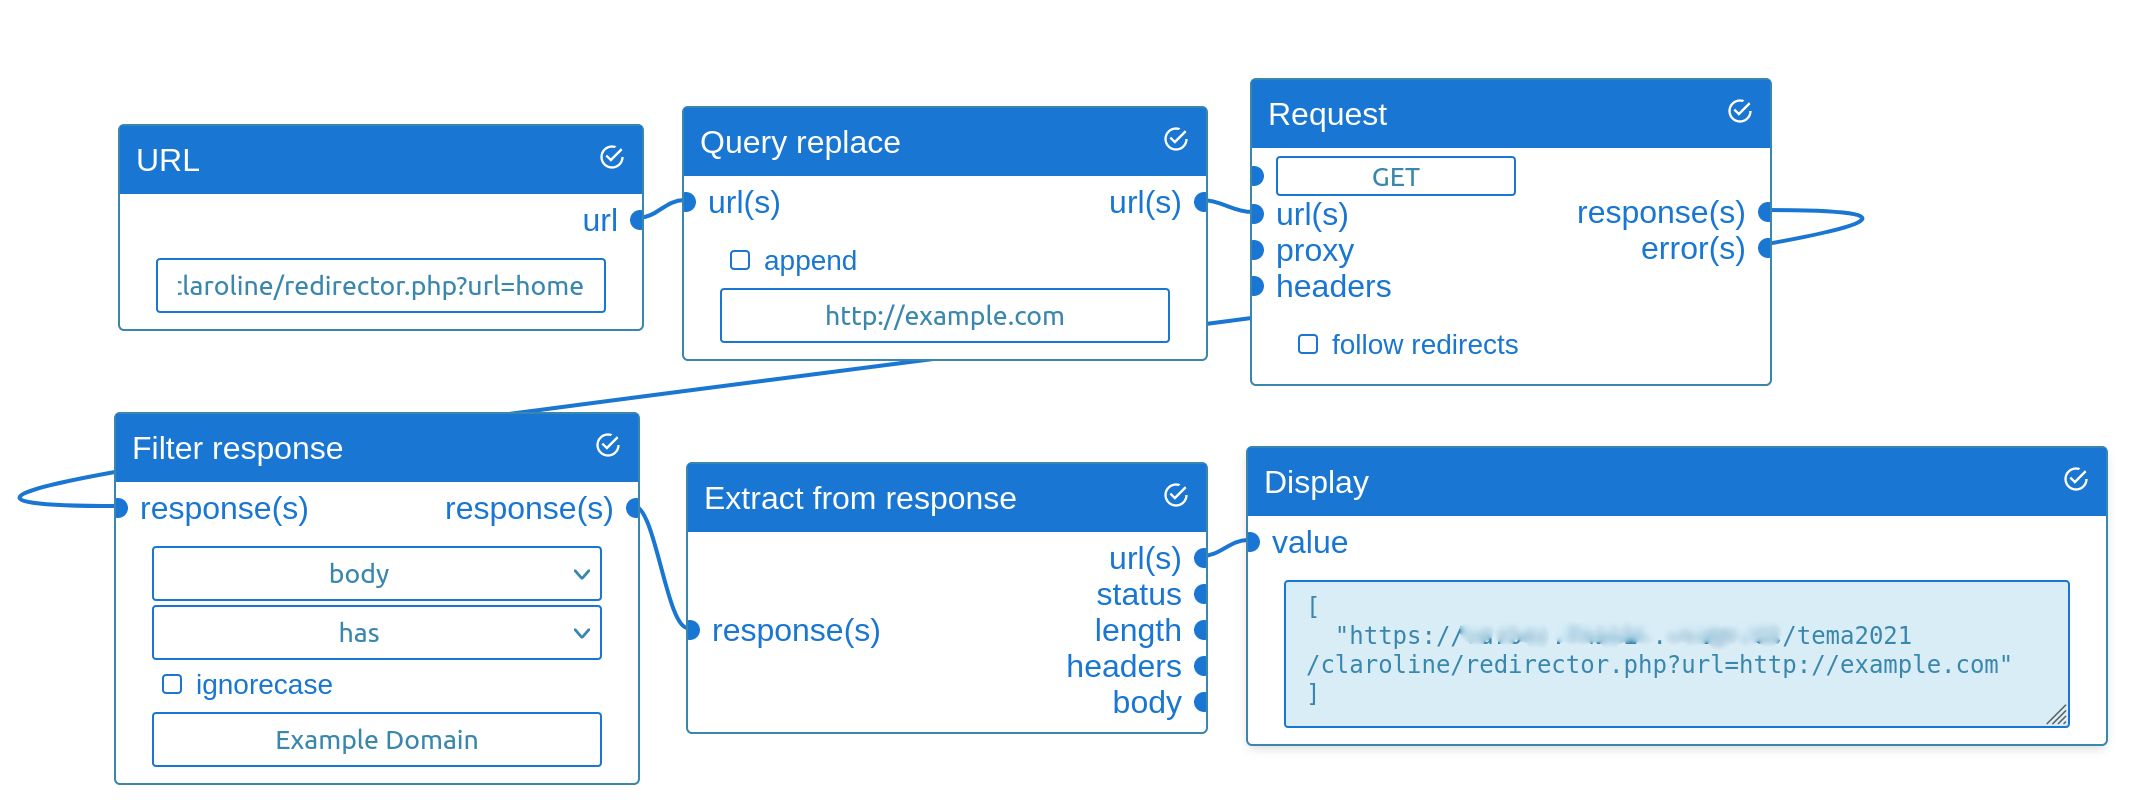
\includegraphics[width=15cm]{img/tables/43_Recipe-OpenRedirect.png}
    \caption{Receta: Vulnerabilidad \textit{OpenRedirect}.}
    \label{fig:openredirect}
\end{figure}

\subsection{Llamadas a la \textit{API}} \label{sub:apicalls}

Al tratarse de un servicio web, es posible realizar llamadas a la \textit{API} sin necesidad de hacer uso de la interfaz. Esta opción está enfocada en los usuario más avanzados que requieran automatizar su flujo de trabajo mediante \textit{scripts}.\sn

Para ello, es necesario realizar una petición \textit{HTTP} usando el método \textit{POST}. Además, la petición debe incluir la cabecera ``\textit{X-Powered-By: Masterchef!}'' y enviar la consulta en formato \textit{JSON}.\sn

Las peticiones actualmente soportadas son\footnote{Los \textit{endpoints} se encuentran detallados en profundidad en el archivo \textit{swagger.yml}}:

\begin{table}[H]
    \begin{center}
        \begin{tabularx}{\textwidth}{| l | l | X |}
            \hline
            \multicolumn{3}{c}{ \textbf{/api/v1/request} } \\
            \multicolumn{3}{c}{Realiza peticiones \textit{HTTP}} \\ \hline
            \textbf{Parámetro} & \textbf{Tipo} & \textbf{Descripción} \\ \hline
            urls & array[url] & Listado de \textit{URLs} objetivo \\ \hline
            method & string & Verbo \textit{HTTP} \\ \hline
            proxy & url & Proxy por el cual enviar las consultas \\ \hline
            headers & map[string]string & Cabeceras \textit{HTTP}. \\ \hline
        \end{tabularx}
    \end{center}
    \caption{\textit{Endpoint} /request}
    \label{tab:endpointrequest}
\end{table}

\begin{table}[H]
    \begin{center}
        \begin{tabularx}{\textwidth}{| l | l | X |}
            \hline
            \multicolumn{3}{c}{ \textbf{/api/v1/lookup/dns} } \\
            \multicolumn{3}{c}{Realiza consultas inversas de \textit{DNS}} \\ \hline
            \textbf{Parámetro} & \textbf{Tipo} & \textbf{Descripción} \\ \hline
            ips & array[ip] & Listado de \textit{IPs} \\ \hline
        \end{tabularx}
    \end{center}
    \caption{\textit{Endpoint} /lookup/dns}
    \label{tab:endpointdns}
\end{table}

\begin{table}[H]
    \begin{center}
        \begin{tabularx}{\textwidth}{| l | l | X |}
            \hline
            \multicolumn{3}{c}{ \textbf{/api/v1/lookup/ips} } \\
            \multicolumn{3}{c}{Realiza consultas de \textit{IP}} \\ \hline
            \textbf{Parámetro} & \textbf{Tipo} & \textbf{Descripción} \\ \hline
            domains & array[domain] & Listado de dominios \\ \hline
        \end{tabularx}
    \end{center}
    \caption{\textit{Endpoint} /lookup/ips}
    \label{tab:endpointips}
\end{table}

\begin{table}[H]
    \begin{center}
        \begin{tabularx}{\textwidth}{| l | l | X |}
            \hline
            \multicolumn{3}{c}{ \textbf{/api/v1/stealth/spider} } \\
            \multicolumn{3}{c}{Obtiene un listado de activos usando fuentes abiertas} \\ \hline
            \textbf{Parámetro} & \textbf{Tipo} & \textbf{Descripción} \\ \hline
            domains & array[domain] & Listado de dominios \\ \hline
            provider & string & Proveedor de búsqueda \\ \hline
            includeSubdomains & boolean & Incluir subdominios \\ \hline
        \end{tabularx}
    \end{center}
    \caption{\textit{Endpoint} /stealth/spider}
    \label{tab:endpointspider}
\end{table}

\begin{table}[H]
    \begin{center}
        \begin{tabularx}{\textwidth}{| l | l | X |}
            \hline
            \multicolumn{3}{c}{ \textbf{/api/v1/stealth/subdomainer} } \\
            \multicolumn{3}{c}{Obtiene un listado de subdominios usando fuentes abiertas} \\ \hline
            \textbf{Parámetro} & \textbf{Tipo} & \textbf{Descripción} \\ \hline
            domains & array[domain] & Listado de dominios \\ \hline
            provider & string & Proveedor de búsqueda \\ \hline
        \end{tabularx}
    \end{center}
    \caption{\textit{Endpoint} /stealth/subdomainer}
    \label{tab:endpointsubdomainer}
\end{table}

Los servicios disponibles a través de la \textit{API} devuelven el código de estado \textbf{404} si no se ha realizado una petición correcta (error en la ruta, método o cabeceras); \textbf{406}, si no se incluyen los parámetros necesarios; o \textbf{200}, si la consulta se ha realizado correctamente.\sn

La figura \ref{fig:apicall} muestra un ejemplo de petición a través de comandos.\sn

\begin{figure}[H]
    \centering
    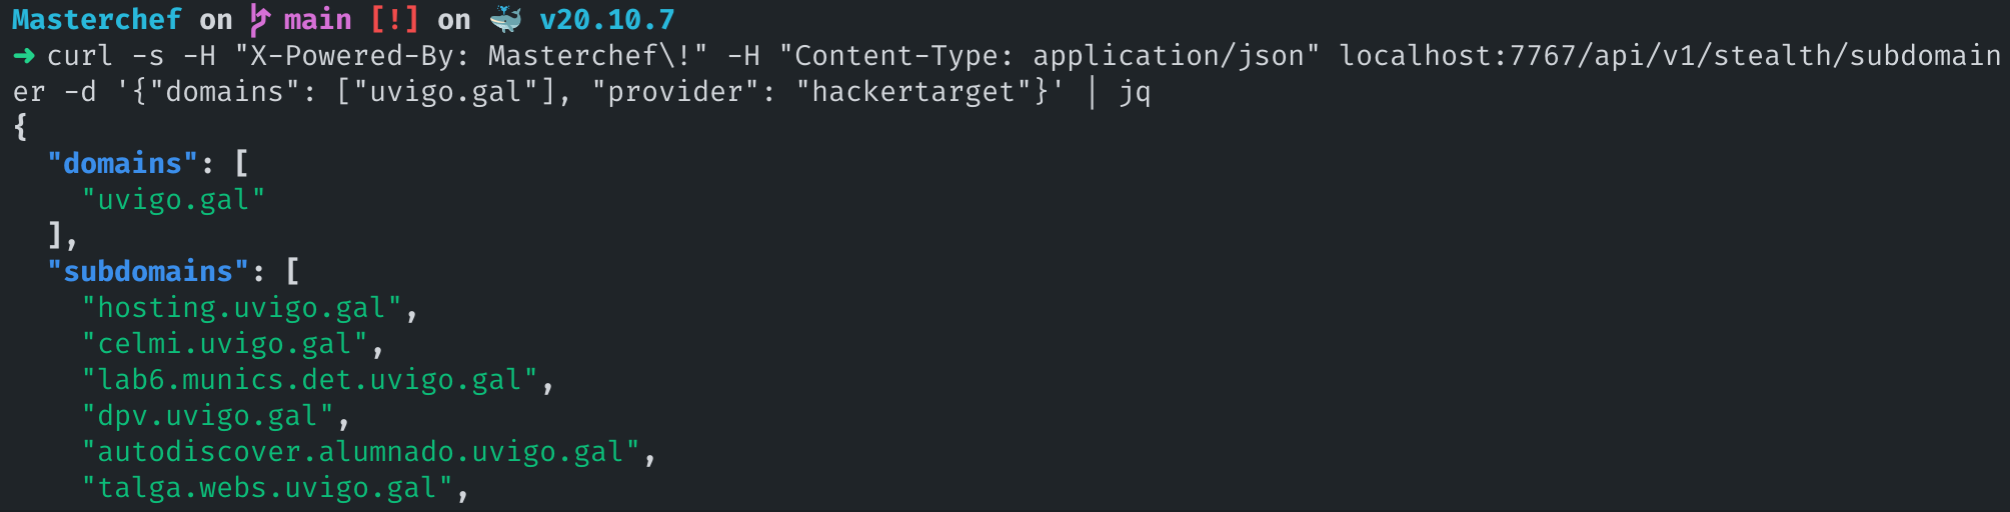
\includegraphics[width=15cm]{img/tables/44_API-Subdomainer.png}
    \caption{Llamada al \textit{subdomainer} a través de \textit{curl}.}
    \label{fig:apicall}
\end{figure}

\newpage

\subsection{Especificación de nuevos \textit{ingredientes}} \label{sub:ingredientspec}

Los tipos de ingredientes están especificados en el archivo \textit{/frontend/src/assets/ingredients.yml}. Actualmente no es posible modificar los ingredientes en soluciones precompiladas. Las especificaciones siguen un formato \textit{YAML}.\sn

Para crear un nuevo tipo de ingrediente, es necesario definir los siguientes valores. Los campos opcionales se marcan con una interrogación (?):\sn

\begin{itemize}
\item \textbf{id}? \ldots Identificador único (sin uso, por el momento).
\item \textbf{name} \ldots Nombre del ingrediente.
\item \textbf{category} \ldots Categoria a la que pertenece.
\item \textbf{aliases} \ldots Etiquetas de búsqueda.
\item \textbf{description} \ldots Descripción de la funcionalidad del ingrediente.
\item \textbf{outputs}? \ldots Conexiones de salida.
    \begin{itemize}
    \item \textbf{name} \ldots Nombre de la conexión.
    \item \textbf{type} \ldots Tipo de la conexión.
    \end{itemize}
\item \textbf{inputs}? \ldots Conexiones de entrada.
    \begin{itemize}
    \item \textbf{name} \ldots Nombre de la conexión.
    \item \textbf{type} \ldots Tipo de la conexión.
    \item \textbf{control}? \ldots Formulario para la modificación de valores por defecto.
        \begin{itemize}
        \item \textbf{type} \ldots Tipo de control.
        \item \textbf{options}? \ldots Valores de configuración del control.
        \end{itemize}
    \end{itemize}
\item \textbf{controls}? \ldots Formularios con los valores de configuración.
    \begin{itemize}
    \item \textbf{name} \ldots Nombre del control.
    \item \textbf{type} \ldots Tipo de control.
    \item \textbf{options}? \ldots Valores de configuración del control.
    \end{itemize}
\item \textbf{code} \ldots Código \textit{JavaScript} para procesar los datos.
\end{itemize}

El campo \textbf{code} cuenta con una serie de variables globales que permiten el acceso a los datos del nodo: \textbf{inputs} (datos de entrada), \textbf{outputs} (datos de salida), \textbf{node.data} (valor de los controles) y \textbf{call} (llamadas a la \textit{API}).\sn

Un ejemplo de especificación de un ingrediente es el mostrado en la figura \ref{fig:ingredientspec}.\n